% -*- mode: LaTeX; coding: utf-8; -*-

\chapter{Tutkimusasetelma}

Edellisissä luvuissa on esitetty osa niistä hyökkäyksistä, joita vastaan verkot ja Web-palvelut joutuvat nykyisin suojautumaan. Niiden suuresta määrästä johtuen on ilmiselvää, että täysin 
turvallista ympäristöä on mahdoton rakentaa. Tätä ei edes pidetä tietoturvasuunnittelun lähtökohtana, vaan tärkeämpää on löytää tasapaino palvelun saatavuuden ja käytettyjen tietoturvaratkaisuiden 
välillä. Liian raskaat menetelmät aiheuttavat ylimääräistä viivettä palvelun tai verkon saatavuuteen, ja liian kevyet ratkaisut jättävät ne avoimiksi tietoturvahyökkäyksille. 

\section{Lähtökohta}
\label{sec:lahtokohta}

Tämän Pro gradu -tutkielman tavoitteena on pyrkiä tunnistamaan Web-palveluihin kohdistuvia poikkeavuuksia analysoimalla palvelimien tallentamaa tapahtumalokia. Analysoitavaksi saamamme loki on 
peräisin yritykseltä, joka tarjoaa hosting-palveluita suuryrityksille. Lokitiedostot ovat peräisin kolmelta tuotannosta jo poistetuilta palvelimilta, ja ne ovat olleet vastuussa muutaman suuren 
palvelukokonaisuuden pyörittämisestä.

Analysoitava data on Apache-palvelimien tuottamaa lokia, joka sisältää
web-palveluille kohdistuvia HTTP-pyyntöjä. Lokia on yhteensä 24
gigatavua, ja se sisältää yli 1,7 miljardia sivupyyntöä.
Lokia on kerätty noin 10 kuukauden
ajanjaksolta. Se on tallennettu \textit{Combined Log Format} -muotoon,
joka on yleinen Apache-palvelimen käyttämä lokitiedoston
muoto~\cite{combined}. Alla on esimerkki onnistuneen HTTP-kyselyn seurauksena muodostuneesta lokirivistä.

% Tarkat luvut:
% - Dataa 24133108 kiB
% - Sivupyyntöjä (ml. error-logit) on 1666171347 kpl.

\begin{framed}
\begin{verbatim*}
130.234.49.2 - - [10/May/2009:15:53:01 +0300]
"GET /scripts/access.pl?user=matti&passwd=admin HTTP/1.1"
200 2680 "http://www.jyu.fi/a.html"
"Mozilla/5.0 (SymbianOS/9.2;...)"
\end{verbatim*}
\end{framed}
\newpage

Web-palvelimien tuottama loki sisältää paljon tietoa muun muassa palveluiden käyttöasteista, ja niihin kohdistuvista kuormista. Niitä analysoimalla voidaan myös tunnistaa mahdollisia hyökkäysyrityksiä, sekä
hyökkäyksen jo tapahduttua tutkia siihen johtaneita vaiheita. Pienillä sivustoilla lokin läpikäyminen jälkikäteen käsin on vielä mahdollista, mutta puhuttaessa palveluista, joilla on miljoonia käyttäjiä 
kuukaudessa, ei tämä ole enää mahdollista. Tästä syystä lokien analysoiminen tulee automatisoida. Tämä taas tarkoittaa sitä, että järjestelmän tulee pystyä tunnistamaan miljoonien kyselyiden joukosta
ne, jotka ovat syntyneet hyökkäyksen johdosta. Yksi mahdollisuus on käyttää sääntöpohjaista ratkaisua, mutta aikaisemmin esitetyistä syistä johtuen ei tämä tarjoa aina riittävää tunnistuskykyä. Tästä 
syystä olemme päätyneet käyttämään anomalioiden tunnistamismenetelmää, jossa järjestelmälle opetetaan normaali käyttäytyminen. Tämän jälkeen haluttua lokia verrataan opetettuun malliin, jolloin poikkeava
liikenne voidaan tunnistaa.

Tietoturvan kannalta kiinnostavin osa logista on GET-parametrin jälkeinen osa, jossa kuljetetaan varsinainen HTTP-pyyntö. Tämä sisältää niin staattiset sivunlatauspyynnöt, kuin myös palvelimelle 
välitettävät parametriarvot. Tällaisia voivat olla esimerkiksi kirjautumisessa käytetyt tiedot, ja tietokannalle välitetyt kyselyt. Staattiset sivunlatauspyynnöt ja parametreja sisältävät pyynnöt erottaa
resurssipolun jälkeisestä kysymysmerkistä. Kysymysmerkin jälkeinen kyselyosuus koostuu avain-arvo-pareista, joista ensimmäinen on kutsuttu parametri, ja jälkimmäinen tämän arvo (kuva \ref{CLF2}). Riippuen
palvelun toteutuksesta näitä voi olla useampia peräkkäin \&-merkillä erotettuna.

\begin{figure}[ht]
\centering
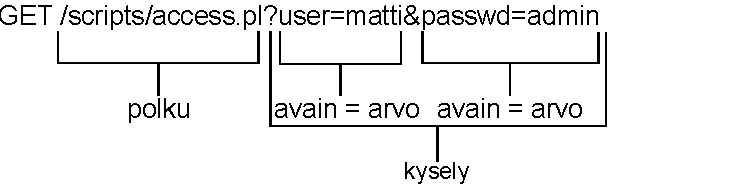
\includegraphics[width=13cm]{pics/logi2.pdf}
\caption{HTTP-kyselyn GET-osa}
\label{CLF2}
\end{figure}

\section{Tutkimuksessa käytetyt menetelmät}

Ongelmia lokin analysoimisessa aiheuttaa sen suuri määrä, ja siinä esiintyvien parametrien tyypit. Parametreista osa on luokka-asteikollisia ja osa puolestaan numeroasteikollisia, joten tietynlaisten toimintamallien 
etsiminen näistä suoraan on haastavaa. Parametrien suuri määrä aiheuttaa myös laskennallisia ongelmia, joten niiden määrää tulee pystyä jotenkin vähentämään säilyttäen kuitenkin mahdollisimman tarkkaan alkuperäisten
muuttujien piirteet. Seuraavaksi esitellään yleisellä tasolla analysoinnissa käytetyt tekniikat, ja tätä seuraa näiden tarkempi matemaattinen kuvaus.

Anomalioiden tunnistamiseen käyttämämme järjestelmä pohjautuu diffuusiokuvausten ja diffuusioetäisyyksien käyttöön. Ne tarjoavat tehokkaan tavan löytää merkittäviä geometrisia rakenteita datasta, ja niiden
käyttämistä moniulotteisen datan esittämisessä on esitelty \cite{diff} \cite{diff2}. Menetelmien tehokkuus perustuu siihen, että diffuusiokuvausten avulla pystytään vähentämään analysoitavan datan dimensioita
säilyttäen kuitenkin sen rakenne. Periaatteessa dimensioiden vähentäminen tarkoittaa sitä, että datajoukko esitetään toisella datajoukolla, jonka dimensio on pienempi. Tällöin sen klusteroiminen sekä 
analysoiminen ja esittäminen graafisesti on helpompaa.

Datan luonteesta johtuen pelkkä dimensioiden vähentäminen ei tuo esille poikkeavuuksia, vaan tätä varten tarvitaan parametreja, jotka kuvaavat HTTP-pyynnön sisältöä tarkemmin. Suurimmasta osasta kyselyn
sisältämistä parametreista kuten IP-osoitteesta, ajasta tai käytetystä selaimesta tämä ei käy ilmi. Toki näistä voidaan tunnistaa esimerkiksi hyökkäykset, joissa yritetään kuluttaa palvelimen resurssit loppuun
hakemalla samaa resurssia yhä uudestaan tai pommittamalla uusia yhteysyrityksiä. Web-palveluihin kohdistuvat hyökkäykset ovat kuitenkin usein paljon hienovaraisempia. Parhaiten näitä voidaan yrittää tunnistaa
tutkimalla tarkemmin GET-parametrin jälkeistä osaa, josta käy ilmi parametrit, joita hyökkääjä välittää palvelimelle. 

Dimensioiden vähentäminen tapahtuu laskemalla diffuusioetäisyydet eli keskimääräiset arvot kaikista kahden pisteen välisistä poluista ts. todennäköisyydet kulkea satunnaiskululla pisteestä toiseen kiinteällä
askelmäärällä. Ennen tätä analysoitava data tulee muuttaa kategoriseksi, sillä muuten erilaisten parametrityyppien välisiä etäisyyksiä ei pystyä laskemaan. Osa parametreista on jo valmiiksi kategorisessa 
muodossa, mutta numeerinen data tulee erikseen kategorisoida. Numeerisen datan automaattinen kategorisointi tapahtuu klusteroimalla yhtä ominaisuutta, ja laskemalla klusteroinnin hyvyysarvo. Tätä jatketaan niin pitkään,
kunnes optimaalinen klusterointi on saavutettu. Prosessi toistetaan vaihtaen kategorioiden lukumäärää jokaisessa iteraatiossa, ja se luku, joka tuottaa parhaimman arvon, valitaan optimaaliseksi kategorioiden 
määräksi .

Tietoturvahyökkäyksissä hyökkääjä pyrkii aina ohittamaan jollakin tavalla asetetut suojaukset. Usein tämä tarkoittaa sitä, että palvelimelle välitetyt pyynnöt muodostuvat pitkistä merkkijonoista, ja niissä käytetyt
merkit poikkeavat tyypillisesti käytetyistä merkeistä. Useiden peräkkäisten avain-arvo parien määrä myös saattaa kasvaa reilusti tavallista suuremmaksi. Näiden tunnistamista varten käytämme analyysissa n-gram -analyysiksi
kutsuttua menetelmää. Menetelmällä lasketaan datassa esiintyvien peräkkäisten merkkien tai sanasten esiintyvyystiheyksiä. Analyysi voidaan tehdä esimerkiksi koko kyselylle, avain-arvo -pareille tai avainten nimille. 

Suurilla tietomassoilla n-gram -analyysi tuottaa isoja matriiseja, joiden käsitteleminen on hidasta. Tehokkuuden takia matriisien ulottuvuuksia tulee pystyä jollakin tavalla vähentämään. Tämä onnistuu satunnaisprojektion 
avulla, joka on ulottuvuuksien vähentämiseen tarkoitettu menetelmä. Satunnaisprojektiossa moniulotteinen data heijastetaan pienempiulotteiseen aliavaruuteen käyttäen satunnaisesti luotua matriisia. Näin syntynyt uusi 
matriisi on laskennallisesti tehokas, ja se säilyttää tässä tapauksessa riittävän määrän informaatiota. 

\subsection{Diffuusiokuvaus}

\todo{Matemaattista oikeellisuutta ei ole vielä tarkistettu!}

Moniulotteisen datan analysoiminen on aina haasteellinen tehtävä johtuen suuresta parametrimäärästä. Tämän takia käytämme tässä työssä hyödyksi diffuusiokuvauksia, jotka ovat tehokas tapa vähentää analysoitavan datan
ulottuvuuksia säilyttäen kuitenkin datan rakenne. Tämän jälkeen sen klusterointi ja visualisointi pienempiulotteisessa avaruudessa on helpompaa.

Ensimmäiseksi diffuusiokuvausiin perustuvalle järjestelmälle opetetaan datan normaali käyttätyminen. Tämä tapahtuu käyttäen opetusmateriaalia, joka on osa analysoitavaa dataa. Olkoot tämä opetusmateriaali 
$\Gamma = \left\{ x_1, x_2, \dots , x_N \right\}, x_i \in \mathbb{R}^n$, jossa $N$ on kyselyiden määrä ja $n$ alkuperäisen datan ulottuvuuksien määrä. Meidän tapauksessa data muodostaa $N \times n$ matriisin, jossa 
rivit pitävät sisällään yksittäiset kyselyt, ja sarakkeet ovat näiden analysoitavat parametrit.

Aluksi luodaan samankaltaisuusmatriisi, joka kuvaa pisteiden välisiä etäisyyksiä käyttäen gaussin jakaumaa. Naapureiden samankaltaisuuden määrittää $\epsilon$. 

\begin{equation}
W_{ij} = e^{-\frac{||x_i - x_j||^2}{\epsilon}}
\label{KERNEL}
\end{equation}

Näin luodun matriisin rivit normalisoidaan diagonaalimatriisin $D$ avulla, joka luodaan yhtälössä \ref{ROWSUM}. 

\begin{equation}
D_{ii} = \sum_{j=1}^{N} W_{ij}
\label{ROWSUM}
\end{equation}

Nyt jokaisen rivin summaksi tulee 1. Tätä normalisointia eli todennäköisyyttä siirtyä tilasta toiseen kuvatkoot $P$

\begin{equation}
P = D^{-1} W
\label{PROB}
\end{equation}

$P$:n ominaisvektorit ovat samat kuin konjugaattimatriisin, joka on esitetty yhtälössä \ref{SYMM}. 

\begin{equation}
\tilde{P} = D^{\frac{1}{2}} P D^{-\frac{1}{2}}
\label{SYMM}
\end{equation}

Jos vaihdamme $P$:n yhtälöstä \ref{SYMM} yhtälössä \ref{PROB} olevan kanssa, saamme yhtälön \ref{NGL} todennäköisyysmatriisin $\tilde{P}$. Näin luotu matriisi säilyttää ominaisvektorien arvot, ja sitä kutsutaan
normalisoiduksi Laplace muunnokseksi.

\begin{equation}
\tilde{P} = D^{\frac{1}{2}} P D^{-\frac{1}{2}} = D^{\frac{1}{2}} D^{-1} W D^{-\frac{1}{2}} = D^{-\frac{1}{2}} W D^{-\frac{1}{2}}
\label{NGL}
\end{equation}

Tämän jälkeen symmetrinen matriisi hajoitetaan käyttäen SVD:tä (engl. Singular Value Decomposition). Koska $\tilde{P}$ on normaali matriisi, spektriteorian (spectral theorem) mukaan tällaisen matriisin 
hajoitelma on yhtälön \ref{SVD} mukainen.  

\begin{equation}
\tilde{P} = U \Lambda U^*
\label{SVD}
\end{equation}

Matriisin $\Lambda$ diagonaalilla olevat arvot ovat samat kuin matriisissa $\tilde{P}$, koska se on symmetrinen. Edelleen koska $\tilde{P}$ on konjugaatti $P$:n kanssa, sisältävät nämä kaksi samat ominaisvektorit 

Matriisin $U = [ u_1, u_2, \dots, u_k ]$ sarakkeet sisältävät matriisin $\tilde{P}$ $k$ ominaisvektoria $u_k$. Käyttämällä yhtälöä \ref{EIGENVECTORS}, voime laskea matriisin $P$ oikeat ominaisvektorit $v_k$, jolloin 
saamme ne matriisin $V$ sarakkeina  $V = [v_1, v_2, \dots, v_k]$.  

\begin{equation}
V = D^{-\frac{1}{2}} U
\label{EIGENVECTORS}
\end{equation}

Nyt datan koordinaatit pienennetyssä ulottuvuudessa ovat yhtälön \ref{MAP_COORDINATES} matriisissa $\Psi$. 

\begin{equation}
\Psi = V \Lambda
\label{MAP_COORDINATES}
\end{equation}

Käyttämällä sopivaa $\epsilon$ spektrin hajoaminen on nopeaa, jolloin riittävän tarkkaan diffuusiokuvaukseen tarvitaan ainoastaan $d$ komponenttia. Ensimmäinen ominaisvektori $V_0$ on vakio, joten se voidaan jättää pois.
Käyttäen ainoastaan ensimmäiset $d$ komponenttia diffuusiokuvauksessa on esitetty yhtälössä \ref{DM}.

\begin{equation}
\Psi_d : x_i \to \left[ \lambda_1 V_{i1}, \lambda_2 V_{i2}, \dots, \lambda_d V_{id} \right]
\label{DM}
\end{equation}

Tämä diffuusiokuvaus upottaa tunnetut pisteet $x_i$ $d$-ulotteiseen avaruuteen. Näin ollen datan uusi ulottuvuus on $n$ vanhan $d$ sijaan.

\subsection{$N$-gram -analyysi}

Koska haluamme analysoida tarkemmin GET-parametrin jälkeistä kyselyosuutta, tarvitsemme tähän menetelmän, joka toimii nopeasti ja tehokkaasti. $N$-gram -analyysi on hyvin tunnettu ja käytetty menetelmä, jolla tutkitaan 
peräkkäisten merkkien tai sanasten esiintymistiheyttä. Sitä käytetään laajalti muun muassa tilastollisen kielen analyysissa, jossa esimerkiksi puheentunnistuksessa sillä tutkitaan foneemeja eli kielen äänneyksikköjä. 

Meidän tapauksessa tutkittavat yksiköt ovat merkkejä, joiden esiintymistiheyttä ja jakaantumista analysoidaan. Merkkien $n$-gram lasketaan käyttäen $n$ pituista liukuvaa ikkunaa. Esimerkiksi sanan ``automaatti'' 2-gram 
saadaan aloittamalla analyysi ensimmäisestä kirjaimesta ja liuttumalla ikkunaa yhden kirjaimen verran. Tässä tapauksessa syntynyt merkkijakauma on ``au'', ``ut'', ``to'', ``om'', ``ma'', ``aa'', ``at'', ``tt'', ``ti''. 
Käyttäen tällä tavoin syntynyttä sarjaa saadaan rakennettua matriisi, joka sisältää tiedon merkkien jakaantumisesta.

$N$-gram -analyysin tuottamien matriisien ulottuvuus on $m^n$, jossa $m$ on datassa esiintyvien sanasten määrä ja $n$ on n-gram -sarjan pituus. Tutkimuksessa analysoidaan vain kahden peräkkäisen merkin esiintyvyyksiä, 
jolloin $n=2$, ja koska tutkittavat sanaset ovat 8-bittisiä merkkejä, niin $m=2^8=256$. Ulottuvuuksia pystytään vähentämään jonkin verran poistamalla sellaiset ulottuvuudet, joissa jokaisessa vektorissa esiintyisi vain 
nollia. Tästäkin huolimatta matriisit ovat niin moniulotteisia, että ulottuvuuksien määrä tulee pystyä jollakin tavoin vähentämään. 

\subsection{Satunnaisprojektio}

Satunnaisprojektiossa alkuperäinen $N$-ulotteinen data heijastetaan $k$-ulotteiseen $(k \ll N)$ aliavaruuteen käyttäen satunnaista $k \times N$ matriisia $R$ \cite{Random}. Olkoot meillä esimerkiksi matriisi 
$X_{m\times N}$, jossa $m$ on havaintojen määrä, ja $N$ on datan alkuperäinen dimensio. Olkoot  $k$  sitten uusi haluttu dimensioiden määrä. Uuden matriisin laskemiseksi luodaan satunnainen matriisi 
$R_{n \times k}$, jossa jokaisen sarakkeen arvot ovat satunnaisesti jakautuneet. Kertomalla nämä keskenään saadaan matriisi $X_{m \times k}^{RP}$, joka on esitys alkuperäisestä datasta $X$ heijastettuna $k$-ulotteiseen 
aliavaruuteen:

\begin{equation}
X_{m \times k}^{RP} = X_{m \times N} \cdot R_{n \times k}.
\label{RP}
\end{equation}

Satunnaisprojektion idea on lähtöisin Johnson-Lindenstrauss lemmasta: jos vektoriavaruudessa olevat pisteet heijastetaan satunnaisesti valittuun aliavaruuteen jossa on sopiva määrä ulottuvuuksia, säilyvät pisteiden
väliset etäisyydet riittävällä tarkkuudella. $X_{m \times N} \cdot R_{n \times k}.$ laskemisen aikavaativuus on $O(dkN)$, ja jos matriisi $X$ sisältää pääasiallisesti nollia ja rivissä on keskimääräisesti $c$ kappaletta arvoja 
$(c \ll N)$, on aikavaativuus $O(ckN)$.

Satunnaisesti luotu matriisi $R$ voidaan valita monella eri tapaa. Useimmiten matriisin $R$ elementit $r_{ij}$ noudattavat Gaussin jakaumaa, mutta se voidaan muodostaa myös muulla tavoin kuten esimerkiksi

\begin{equation}
r_{ij} = \sqrt{3}\cdot 
\begin{cases}
 +1 &\text{todennäköisyydellä $\frac{1}{6}$} \\
 0 &\text{todennäköisyydellä $\frac{2}{3}$} \\
 -1 &\text{todennäköisyydellä $\frac{1}{6}$} \\
\end{cases}
\label{RPChoice}
\end{equation}

Tällaisen jakauman käyttäminen vähentää entisestään laskenta-aikaa, sillä laskenta voidaan suorittaa käyttäen kokonaislukuja. Yllä olevan jakauman tapauksessa laskenta on vieläkin nopeampaa, sillä operaatioista
tarvitaan vain kolmasosa, sillä luotu matriisi sisältää suurimmaksi osaksi nollia \cite{Random}.

% Tuomon kommentit:
%
% "Dimensioiden vähentäminen tapahtuu" -kappale esittää asian jotenkin
% eri tavalla. Tuo voi tietysti pohjautua Diffusion maps -julkaisuun.
%
% En ole lukenut että asia esitettäisiin noin. Tavallaan se on totta,
% mutta en ole aivan varma voiko sen sanoa noin.
%
% Minusta tuo parametreja käsittelevä kappale voisi olla ennen
% diffuusiokarttaa. Tällöin liikuttaisiin loogisessa järjestyksessä, eli
% ensin piirteiden erottaminen ja sitten vasta niistä muodostuvan
% taulukon ulottuvuuksien vähentäminen.
%
% Viitteitä voisi olla n-grammien käyttöön.
%
% Ainakin miten Juholta olen ymmärtänyt, tuossa mallissa
% diffuusiokarttaa käytetään vain alkuvaiheen koulutusdatan
% suodattimena.
%
% Mutta tuo tuleekin tosiaan esille kun tuohan oli vain yleiskuvaus. Ja
% se voisi minusta olla virtaviivaisempi.
%
% Sanottaisiin, että nyt tehdään X, saadaan tuloksena Y, sitten tehdään
% näin ja saadaan tuloksena tämä... ja lopulta saadaan haluttu tieto
% anomalioista.
%
% Kuvat selventää aina.
%
% Mutta tuo teksti on hieman sekavassa järjestyksessä vielä.
